\section{Scalar multiplication}

\begin{outcome}
  \begin{enumerate}
  \item Multiply a scalar by a vector algebraically and geometrically.
  \item Use the laws of scalar multiplication to prove equalities
    between vector expressions.
  \end{enumerate}
\end{outcome}

Scalar multiplication of vectors in $\R^n$ is defined as
follows.

\begin{definition}{Scalar multiplication of vectors in $\R^n$}{vector-scalar-multiplication}
  If $k\in\R$ is a scalar and $\vect{u}\in \R^n$ is a vector, then
  their \textbf{scalar multiplication}%
  \index{vector!scalar multiplication}%
  \index{scalar multiplication!of a vector} $k\vect{u}\in \R^n$ is
  defined by
  \begin{equation*}
    k\vect{u}=k\begin{mymatrix}{c}
      u_1 \\
      \vdots \\
      u_n
    \end{mymatrix} = \begin{mymatrix}{c}
      ku_1 \\
      \vdots \\
      ku_n
    \end{mymatrix}.
  \end{equation*}
\end{definition}

For example $3 \mat{1, 2, 3}^T = \mat{3, 6, 9}^T$ and
$-2\mat{1, 2, 3}^T = \mat{-2, -4, -6}^T$.

\begin{example}{Geometric meaning of scalar multiplication}{geometric-scalar-multiplication}
  Let $\vect{u}=\mat{2,1}^T$, and draw the following vectors to scale:
  $2\vect{u}$, $\vect{u}$, $\frac{1}{2}\vect{u}$, $0\vect{u}$,
  $-\frac{1}{2}\vect{u}$, $-\vect{u}$, and $-2\vect{u}$.  What is the
  geometric meaning of scalar multiplication?
\end{example}

\begin{solution}
  Here is a picture of the seven vectors. We draw their tails in
  different places to make their relationship easier to see.
  \begin{center}
    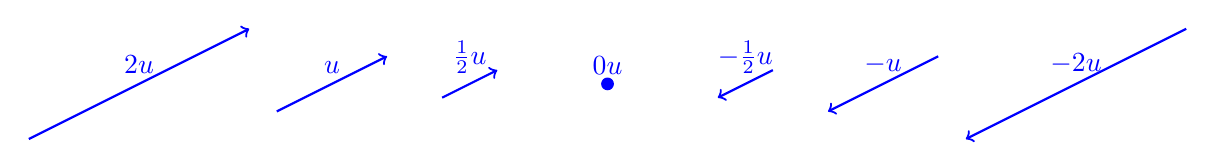
\begin{tikzpicture}[scale=0.7]
      \draw[->, thick, blue] (-10.5,-1)    -- node[above]{$2\vect{u}$} +(4,2);
      \draw[->, thick, blue] (-6,-0.5)  -- node[above]{$\vect{u}$} +(2,1);
      \draw[->, thick, blue] (-3,-0.25) -- node[above]{$\frac{1}{2}\vect{u}$} +(1,0.5);
      \draw[fill, blue](0,0) circle [radius=3pt] node[above]{$0\vect{u}$};
      \draw[->, thick, blue] (3,0.25)   -- node[above]{$-\frac{1}{2}\vect{u}$} +(-1,-0.5);
      \draw[->, thick, blue] (6,0.5)    -- node[above]{$-\vect{u}$} +(-2,-1);
      \draw[->, thick, blue] (10.5,1)      -- node[above]{$-2\vect{u}$} +(-4,-2);
    \end{tikzpicture}
  \end{center}
  We see that the vector $k\vect{u}$ has the same direction as
  $\vect{u}$ when $k$ is positive, and the opposite direction when $k$
  is negative. Further, the length of the vector is scaled by a factor
  of $\abs{k}$. It increases if $\abs{k}>1$ and decreases if
  $\abs{k}<1$. For example, the vector $2\vect{u}$ is exactly twice as
  long as $\vect{u}$.  (It is because of this scaling property that
  scalars are called scalars%
  \index{scalar!for scaling}).
\end{solution}

Just as with addition, scalar multiplication of vectors satisfies
several important properties. These are outlined in the following
proposition.

\begin{proposition}{Properties of scalar multiplication}{vector-scalar-multiplication}
  The following properties hold for vectors
  $\vect{u},\vect{v}\in\R^n$ and $k,\ell$ scalars.%
  \index{vector!properties of scalar multiplication}%
  \index{vector!scalar multiplication!properties}%
  \index{properties of scalar multiplication!vector}%
  \begin{itemize}
  \item The distributive law over vector addition
    \index{distributive law!over vector addition}%
    \index{vector!distributive law}%
    \begin{equation*}
      k(\vect{u} + \vect{v}) = k\vect{u} + k\vect{v}.
    \end{equation*}
  \item The distributive law over scalar addition
    \index{distributive law!over scalar addition}%
    \begin{equation*}
      (k + \ell) \vect{u} = k\vect{u} + \ell\vect{u}.
    \end{equation*}
  \item The associative law for scalar multiplication
    \index{associative law!of scalar multiplication}%
    \index{vector!associative law of scalar multiplication}%
    \begin{equation*}
      k(\ell\vect{u}) = (k\ell)\vect{u}.
    \end{equation*}
  \item The rule for multiplication by $1$
    \index{rule for multiplication by 1}%
    \index{vector!rule for multiplication by 1}%
    \begin{equation*}
      1\vect{u}=\vect{u}.
    \end{equation*}
  \end{itemize}
\end{proposition}

\begin{proof}
  We will show the proof of:
  \begin{equation*}
    k(\vect{u} + \vect{v}) = k\vect{u} + k\vect{v}.
  \end{equation*}
  Assume $\vect{u}=\mat{u_1,\ldots,u_n}^T$ and
  $\vect{v}=\mat{v_1,\ldots,v_n}^T$. We have:
  \begin{equation*}
    \begin{array}{ll}
      k(\vect{u} + \vect{v}) & = k\mat{u_1 + v_1,\ldots,u_n + v_n}^T \\
                             & = \mat{k(u_1 + v_1), \ldots, k(u_n + v_n)}^T \\
                             & = \mat{ku_1 + k v_1, \ldots, ku_n + kv_n}^T \\
                             & = \mat{ku_1, \ldots, ku_n}^T + \mat{kv_1, \ldots, kv_n}^T \\
                             & = k\vect{u} + k\vect{v}.
    \end{array}
  \end{equation*}
\end{proof}

